%% Papier complet HCII 2027 (EPCE), tire de la seconde proposition (papers/HCII27_Miroir/proposition-hcii2027.md).
%% Echeance annoncee : 29 janvier 2027, 10 a 20 pages LNCS. A VERIFIER sur la page officielle avant le depot.
%% Chaque chiffre est recalcule par verify_sections.py (carnet HCII27_Miroir_statistics.ipynb) ; ne pas en ajouter sans controle.
%% Aucun tiret cadratin.

\documentclass[runningheads]{llncs}
\usepackage[T1]{fontenc}
\usepackage[utf8]{inputenc}
\usepackage{lmodern}
\usepackage{microtype}
\usepackage{graphicx}
\usepackage{booktabs}
\usepackage{amsmath}
\usepackage{multirow}
\usepackage[hyphens]{url}

%% Flottants : le tableau des criteres est haut ; avec les reglages par defaut il partait APRES les references, et le tableau 3 derriere
%% lui (vu sur les vignettes du 10 nov. 2026, aucun compteur ne l avait signale).
\renewcommand{\topfraction}{0.92}
\renewcommand{\bottomfraction}{0.6}
\renewcommand{\textfraction}{0.06}
\renewcommand{\floatpagefraction}{0.85}
\setcounter{topnumber}{3}
\setcounter{bottomnumber}{2}
\setcounter{totalnumber}{5}

\begin{document}

\title{A Pilot That Learns and a Twin That Watches:\\Testing a Cognitive Pilot Model\\Against Pilots It Has Never Seen}
\titlerunning{A Pilot That Learns and a Twin That Watches}

\author{Daril Kengne Wambo \and Vanessa Mankejeu Ngolong \and Roger Nkambou}
\authorrunning{D. Kengne Wambo et al.}
\institute{Centre de recherche en intelligence artificielle (CRIA),\\
Universit\'e du Qu\'ebec \`a Montr\'eal, Montr\'eal QC H2X 3Y7, Canada\\
\email{kengne\_wambo.daril\_raoul@courrier.uqam.ca}}

\maketitle

\begin{abstract}
Flight instructors judge a trainee from the seat behind, one flight at a time. A digital twin of the pilot could follow every flight
against the written procedure and anticipate the trainee's next actions, provided it can do so for a pilot it has never seen. We test
this on VC-PILOT, an ACT-R pilot whose procedures are held as declarative knowledge drawn from a procedure ontology. Read in reverse,
the same knowledge becomes a mirror that recognises which step of the procedure a pilot is executing; run twenty seconds ahead of the
aircraft, it becomes a twin that predicts when the pilot's next actions will come. On 211 simulator take-offs by twelve pilots, nominal
and with engine failures, the mirror recognised all 1,686 pilot actions found offline, with a median lag of 0.08\,s. Predicting each
pilot from that pilot's earlier flights alone, with everything else learned from the other eleven, the twin came closer to the pilot's
actual timing than the pilot's own record did for 11 of 12 pilots, by 1.0\,s at a 20\,s horizon, and closer than the strongest
baseline that follows the flight without a cognitive model for 9 of 12, by 0.32\,s (95\,\% interval 0.12 to 0.57), an advantage
carried by the cognitive model itself. At 10\,s it is not established. The pacing of routine actions proved to be a personal signature, with intraclass correlations of 0.71 to
0.80, while the response to a failure was not, which bounds what an expectation-based monitor can flag. Each pre-registered criterion
we discuss is reported with its verdict, failures included.

\keywords{Cognitive digital twin \and ACT-R \and Pilot modelling \and Individual differences \and Pre-registration \and Flight simulation}
\end{abstract}

%% ====================================================================================================
\section{Introduction}

In flight training the instructor is the measuring instrument. Seated behind the trainee, the instructor follows the procedure step by
step, notices that the gear came up late or that the flaps were retracted early, and anticipates the next mistake before it happens.
Simulators record every flight, but a recording does not say which step of the procedure the trainee was on, whether an action came
late, or what the trainee was about to do. Those are the questions an instructor answers, and they are what a digital twin of the pilot
would have to answer to be of use to a training organisation.

Such a twin has to meet three demands. It must \emph{follow} a pilot's flight closely enough to name the step being executed. It must
\emph{anticipate} the timing of the pilot's next actions, since a missing action can only be flagged once it is overdue. And it must do
both for a pilot it has \emph{never seen}, because a trainee is new by definition. A fourth demand concerns the model behind the twin
rather than the twin itself: if the same model is to stand in for trainees when a procedure or a cockpit is redesigned, its skill should
improve with practice the way a person's does.

Cognitive architectures have flown aircraft in simulation for a long time~\cite{jones_tacair_1999,zemla_2011_actr_taxiing}, and some
have been compared with pilots~\cite{xu_computational_2024}. The comparison is usually made on group averages, and the few models that
follow individual pilots trace their behaviour in specific situations, such as their response to an alert~\cite{klaproth_neuroadaptive_2020,blum_anticipation_2022}.
A twin is judged differently: on one person at a time, over whole procedures, and against a demanding alternative. Whatever a cognitive model predicts about a pilot, one could also predict from that pilot's own past flights, or
from the events of the current flight, without any cognitive model at all. A twin earns its keep only if it does better than these.

We build on VC-PILOT~\cite{kengne_cpilot_2026}, an ACT-R pilot~\cite{anderson2004integrated} whose procedures are not written as
production rules but held as declarative knowledge, read from a procedure ontology~\cite{courtemanche_ontological_2022} by a small,
fixed set of generic rules. Because the procedure is data, the same knowledge can be used three ways: to fly the aircraft, to read a
pilot's flight against the procedure (the \emph{mirror}), and to run ahead of the aircraft and say what the pilot will do next (the
\emph{twin}). We ask four questions. Does the skill the model acquires through practice match pilots it was never tuned on? Can the
mirror follow a pilot's flight? Does the twin anticipate a pilot better than the pilot's own record, and better than a strong
statistical baseline that knows what has already happened in the flight? And what, in an individual pilot's timing, is predictable at
all?

The paper makes four contributions. First, a mirror that reads a pilot's flight through the knowledge the agent flies with, so that a
deviation is reported against a named step of the procedure rather than as an anomaly score. Second, a pilot-by-pilot evaluation of the
twin against the pilot's own record and against the strongest baseline we could build without a cognitive model, in which each pilot is
predicted from earlier flights only and everything else is learned from the other pilots; looking twenty seconds ahead, the advantage
belongs to the cognitive model itself. Third, the observation that the pacing of routine actions is a stable personal signature while
the response to a failure is not, and what this implies for training and for monitoring. Fourth, a record of pre-registered criteria
with their failures: the model's learning plateaued against held-out pilots, and alerts on omitted
actions fell short of their target. Every criterion was written, with its threshold, and time-stamped in version control before it was
computed~\cite{nosek_preregistration_2018}; amendments are dated, and a failure is never removed by a change made to pass it.

%% ====================================================================================================
\section{Related Work}

\paragraph{Cognitive pilots.} TacAir-Soar, a rule-based system built in Soar~\cite{laird2012soar}, flew most of the fixed-wing missions
of the United States military in large simulated exercises~\cite{jones_tacair_1999}. In ACT-R~\cite{anderson2004integrated,ritter2019actr},
a model of commercial jetliner taxiing flew among aircraft replayed from recordings of a real airport, so that its trajectories could be
compared with those of pilots~\cite{zemla_2011_actr_taxiing}; QN-ACTR extended the architecture toward multitask
performance~\cite{cao_queueing_2013_qnactr}. Xu and colleagues compared two models of pre-flight and take-off with pilots flying the
same tasks in a simulator, with errors of 0.8 to 13.2\,\% on performance and workload~\cite{xu_computational_2024}. Kotseruba and
Tsotsos review what such architectures can and cannot yet do~\cite{kotseruba_40years_2020}. Our earlier work moved a pilot's procedures
out of production rules into a procedure ontology, so that one interpreter flies different aircraft~\cite{kengne_cpilot_2026}. Closest
to our question, Klaproth and colleagues traced individual pilots' responses to flight-deck alerts with an ACT-R model informed by
EEG~\cite{klaproth_neuroadaptive_2020}, and Blum and colleagues anticipated the actions of thirteen pilots with an ACT-R model that
represents individual differences~\cite{blum_anticipation_2022}. To our knowledge, no such model has been compared, pilot by pilot and
with each pilot held out, against the pilot's own record and against a baseline that follows the flight, as a predictor of when the
next actions will come. That is the test we apply here.

\paragraph{Skill acquisition.} Production compilation turns the slow interpretation of declarative instructions into fast task-specific
rules~\cite{taatgen_lee_2003}; threaded cognition explains how concurrent tasks share the same resources~\cite{salvucci_threaded_2008}.
Both bear on whether a model can improve with practice the way a trainee does, the question of our first test.

\paragraph{Inferring the pilot's state.} Neuroadaptive and assistance systems infer the pilot's mental state from physiology and
behaviour~\cite{klaproth_neuroadaptive_2020,russwinkel_cognitive_assistance_2020}, in the line of work on situation
awareness~\cite{endsley_toward_sa_theory_1995} and workload~\cite{hart_nasa-task_load_2006,wickens_engineering_2021}. ACT-R models have
represented the effect of fatigue on performance~\cite{gunzelmann_sleep_deprivation_2009}. We test whether an estimated state improves
the twin's predictions; it does not (Section~\ref{sec:discussion}).

\paragraph{Individuals and populations.} Predicting an individual from few observations is a classic problem of empirical Bayes: an
individual estimate is shrunk toward the population in proportion to how much individuals actually differ~\cite{efron_morris_1975}. The
same variance decomposition gives the intraclass correlation~\cite{shrout_fleiss_1979}, which we use to ask which parts of a pilot's
timing are personal.

%% ====================================================================================================
\section{One Body of Knowledge, Three Uses}
\label{sec:system}

\subsection{Procedures as declarative knowledge}

A procedure is a set of tasks. Each task carries one or more \emph{actions}, a cockpit parameter and the value it must reach (thrust
levers at take-off thrust, gear lever up), \emph{preconditions} on earlier tasks, and \emph{constraints} on the aircraft's state (a
speed, a height). Tasks belong to a procedure: the normal take-off, the rejected take-off, and the take-off continued after an engine
failure past the decision speed. Table~\ref{tab:glossary} gives the few terms of aviation the paper needs.

A fixed set of 37 generic production rules interprets these tasks~\cite{kengne_cpilot_2026}. They retrieve the next task whose
preconditions hold, wait for its constraints, act, and verify that the action took effect; no rule names a task. Practice changes this
behaviour through two standard ACT-R mechanisms. Production compilation fuses the retrieval of a task and its execution into a
task-specific rule nobody wrote~\cite{taatgen_lee_2003}, and utility learning, driven by a reward at the end of each task, decides when
the compiled rule wins over the generic rules it came from. When a failure is detected, the interpreter switches procedure, for instance
from the normal to the rejected take-off.

\begin{table}[t]
\caption{The aviation terms used in this paper.}
\label{tab:glossary}
\centering\small
\begin{tabular}{@{}p{3.7cm}p{8.1cm}@{}}
\toprule
Term & Meaning \\
\midrule
Brake release & Start of the take-off roll; time zero of a take-off in this paper. \\
Take-off thrust & Thrust levers set to take-off power, after a stabilisation at about 50\,\%. \\
V1 & Decision speed: below it a failure leads to a rejected take-off, above it the take-off continues. \\
Rotation, liftoff & The pilot raises the nose; the wheels leave the ground. \\
Gear up, thrust reduction & Landing gear retracted after liftoff; thrust reduced to climb power at a set height. \\
Flaps 1, flaps 0 & Successive retraction of the wing flaps as speed increases. \\
Rejected take-off & Take-off abandoned on the runway: thrust to idle, reverse thrust, maximum braking. \\
Continued take-off & Take-off pursued on one engine after a failure above V1. \\
\bottomrule
\end{tabular}
\end{table}

\subsection{The mirror: reading a flight against the procedure}

The mirror runs the same knowledge without acting. It reads the aircraft's state, from a recording or live from the simulator, and
writes nothing back. For the task the pilot should be on, it compares each action's parameter with its target; an action counts as
done once the parameter has reached its target and held it for one second, so that a hesitation shorter than a second does not break it.
For every task the mirror logs when it was done and whether it came early, late or not at all with respect to qualified pilots, and when
a failure appears it follows the pilot into the corresponding procedure. Offline, it reads recorded flights; live, an ACT-R model follows
the flight in parallel, as the agent would fly it.

\subsection{The twin: running the model ahead of the aircraft}

The twin makes two kinds of prediction. The first is immediate: when the mirror's model reaches a task, it predicts the pilot's action
at the time the model is ready, plus an offset learned for that pilot. The offset is the pilot's median deviation on earlier flights,
shrunk toward the median of other pilots as
\begin{equation}
J = \frac{n\,\tilde{x}_{\mathrm{pilot}} + K\,\tilde{x}_{\mathrm{others}}}{n + K},
\label{eq:shrink}
\end{equation}
where $\tilde{x}$ denotes a median, $n$ is the number of the pilot's earlier observations, and $K = 16$ was chosen on the calibration
pilots alone. With few flights the pilot is predicted like everyone else; with many, from the pilot's own flights.

The second prediction looks ahead. Every five seconds a copy of the model, reset to the mirror's current position in the procedure, runs
twenty seconds ahead in simulated time. It flies against an aircraft trajectory extrapolated from the five most similar take-offs of other
pilots, and its commands go to a stand-in simulator, never to the real one. The time at which the copy is ready for each task, plus the
pilot's offset for that task, is the twin's prediction. Two further details matter. The recorded flights are timed in simulated seconds, and the simulator in
which the pilots flew ran about 9\,\% slower than the clock, whereas ACT-R's latencies are human seconds; the trajectory is therefore
stretched by the ratio measured on each flight. And the prediction in service is a weighted average,
$H = 0.75\,A + 0.25\,B$, of the model's prediction $A$ and a reference $B$, the pilot's shrunk median delay of the action since brake
release, or since the failure for the actions of a failure procedure; the weight was chosen on calibration pilots. Each prediction
carries an interval meant to contain the action four times out of five, learned on the same pilots; on the validation pilots it
contained 70\,\% of their actions, at the lower edge of the range we had required. Figure~\ref{fig:timeline} shows what the twin said,
ten seconds ahead, during one take-off of a pilot it had not been calibrated on.

The mirror and the twin run live next to the simulator, in a dashboard that shows the step the pilot is on, the predicted time of the
next actions with their intervals, and the actions that are overdue. We have run it in live sessions with our own agent at the
controls; it has not yet watched a human pilot live.

\begin{figure}[t]
\centering
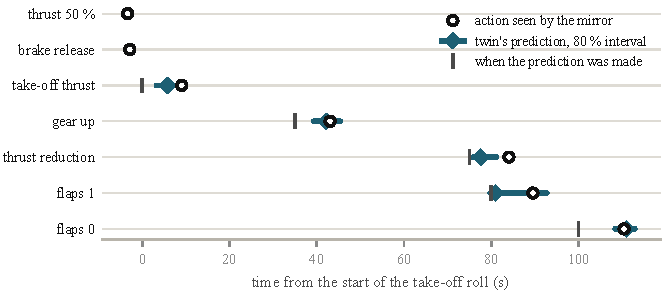
\includegraphics[width=\linewidth]{fig_timeline.pdf}
\caption{One nominal take-off of validation pilot 11. Open circles: actions recognised by the mirror. Diamonds: what the twin predicted
about ten seconds earlier, with its 80\,\% interval; the tick marks when the prediction was made. Four of the five actions fall inside
their interval; the thrust reduction came 2.8\,s after its interval closed. The first two actions precede the roll, when the twin does
not yet predict.}
\label{fig:timeline}
\end{figure}

%% ====================================================================================================
\section{Data and Protocol}
\label{sec:protocol}

\paragraph{Pilots and flights.} Twelve pilots flew take-offs in a fixed-base Airbus A320 simulator: five type-rated airline pilots, two
licensed pilots and five novices. The corpus holds 211 take-offs, 104 nominal, 63 rejected after an engine failure and 44 continued on
one engine; each pilot flew between 4 and 21 of them. The time of each failure is dated from the engines' fuel flows. A separate test of
the learning model used 129 nominal take-offs from the same study. The flight data and the procedure ontology belong to the project's
industrial partners and cannot be released.

\paragraph{Calibration, validation and blindness.} Six pilots (2, 3, 5, 6, 7 and 10) served for calibration, and everything that can be
tuned was tuned on them. The other six (4, 8, 9, 11, 12 and 13) were held out. They were judged blind for the last time on
8~November~2026. Corrections made after that date were judged again on the same pilots, no longer blind, and Table~\ref{tab:criteria}
marks those results as corrected.

\paragraph{Pre-registration.} Before each computation, the criterion, its threshold and our predicted outcome were committed to the
project's repository. When a criterion had to be amended, for instance because a rule of the evaluation was found to be wrong, the
amendment was dated and the first judgement kept.

\paragraph{The pilot's own record, cross-validated.} The comparisons of Section~\ref{sec:own} use every pilot. To judge one pilot, the
other eleven provide everything that is learned, and the pilot is predicted, flight after flight, from earlier flights alone. Where a
prediction uses the pilot's record, it shrinks it toward the other pilots as in Eq.~\ref{eq:shrink}, but with a weight that is estimated
rather than chosen: $K$ is the ratio of within-pilot to between-pilot variance of the quantity, computed on the other eleven pilots by a
one-way analysis of variance on values winsorised at their 5th and 95th percentiles~\cite{efron_morris_1975}. Nothing in this
evaluation is tuned.

\paragraph{Measures.} A prediction is made at time $t$ and judged on the pilot actions that come in the next $h$ seconds, $h = 10$ or
20, leaving out actions that follow a failure the predictor could not yet have seen. All predictors are judged on the same pairs: 1,241
at 10\,s and 1,938 at 20\,s. The error is the median absolute difference between predicted and actual time, per pilot and pooled. We
count the pilots for whom one predictor beats another, with a one-sided sign test, and give a 95\,\% interval for the pooled difference
from 10,000 bootstrap resamples of pilots.

%% ====================================================================================================
\section{Results}
\label{sec:results}

Table~\ref{tab:criteria} lists every pre-registered criterion discussed in this paper with its verdict. We take the four questions in
turn.

\begin{table}[!tp]
\caption{Pre-registered criteria and their verdicts. \emph{Frozen}: protocol frozen before any flight, pilots held out.
\emph{First run}: the first judgement of the criterion. \emph{Corrected}: judged again after a correction, on data already seen.
\emph{Cross-val.}: all twelve pilots, each predicted without being learned from.}
\label{tab:criteria}
\centering\scriptsize
\setlength{\tabcolsep}{3pt}
\begin{tabular}{@{}p{4.45cm}p{1.2cm}p{4.15cm}l@{}}
\toprule
Criterion & Run & Result & Verdict \\
\midrule
\multicolumn{4}{@{}l}{\emph{A pilot that learns: six modelled pilots against six held-out pilots, 60 flights}} \\
Liftoff to gear up matches the pilots & frozen & 11.6\,s against 5.5\,s, difference 6.1\,s (99\,\% interval 4.8 to 7.8) & FAIL \\
Thrust reduction before the first flaps & frozen & 57 of 57 flights against 34 of 35 & PASS \\
Gear up before thrust reduction; omissions; slope of learning & frozen & too few events to decide (8 criteria) & inconclusive \\
Thrust reduction: height and time after liftoff & frozen & 1,581 against 1,700\,ft; 27.0 against 36.4\,s & FAIL \\
\midrule
\multicolumn{4}{@{}l}{\emph{The mirror, replaying all 211 take-offs}} \\
Actions recognised (at least 90\,\%) & first run & 1,680 of 1,686; 1,686 after correction & PASS \\
Median lag (at most 1.5\,s) & first run & 0.21\,s; 0.08\,s after correction & PASS \\
False recognitions (at most 10\,\%) & first run & 4 of 1,684; 1 of 1,687 after correction & PASS \\
\midrule
\multicolumn{4}{@{}l}{\emph{The twin}} \\
Next action: the pilot's offset beats the generic model & first run & 12 of 12 pilots & PASS \\
Next action: beats the other pilots' offset & first run & 6 of 12 pilots & FAIL \\
\quad same, with $K$ set on calibration pilots & corrected & 6 of 6 validation pilots & PASS \\
Twenty seconds ahead: beats reference $B$ in error & first run & 5 of 6 at 10\,s and at 20\,s & PASS \\
\quad and predicts as many actions as $B$ & first run & 0.88 against 0.94 of actions at 10\,s & FAIL \\
\quad after a failure assumed in advance & first run & 2 of 5 pilots & FAIL \\
\quad an estimated cognitive state improves it & corrected & 2 of 6 pilots; $+0.012$\,s & FAIL \\
\midrule
\multicolumn{4}{@{}l}{\emph{The twin against the pilot's own record}} \\
Twin beats the pilot's own record & cross-val. & 11 of 12 at 10 and 20\,s & PASS \\
Twin beats the event baseline & cross-val. & 9 of 12 at 20\,s; 7 of 12 at 10\,s & PASS (20\,s) \\
\quad the model alone, without the blend & cross-val. & 10 of 12 at 20\,s; 7 of 12 at 10\,s & reported \\
Personalising the twin further improves it & cross-val. & 5 of 12; worse by 0.07\,s & FAIL \\
\midrule
\multicolumn{4}{@{}l}{\emph{Flagging a missing action}} \\
80\,\% intervals contain the action (70 to 90\,\%) & corrected & 70\,\% of 983 actions & PASS \\
At most 0.75 false alerts per flight & corrected & 0.09 & PASS \\
Omitted action flagged within 10\,s (80\,\%) & cross-val. & 63\,\% (59\,\% without personalisation) & FAIL \\
\bottomrule
\end{tabular}
\end{table}

\subsection{A pilot that learns, tested on pilots it never saw}

The model learned. In development, one modelled pilot reproduced the shape of the human learning curve: the time from liftoff to gear
up fell from 6.7\,s on its first flight to 3.8\,s on its second, once its compiled rules were reloaded, and then stayed near 3.6\,s;
the pilots go from 15.1 to 5.7 and then 3.3\,s. The frozen test, run on six modelled pilots of ten flights each against the six held-out
pilots, did not confirm it. On the first flight the agent was close to the pilots, 16.1\,s against 15.1\,s, but it then stopped
improving: 11.6\,s on flights 2 to 7 and 11.5\,s on flights 8 to 10, where the pilots reached 6.1 and 3.1\,s. The pre-registered test
of this delay fails. Its cause, among the documented differences between the development and frozen configurations, is not established.
The order of the procedure held: the agent reduced thrust before the first flap retraction in all 57 flights where both occurred, as
the pilots did in 34 of 35, and its rotation speed and peak pitch fell within the pilots' interquartile range. Its thrust reduction, on
the other hand, came earlier and lower than the pilots', at 1,581 against 1,700\,ft, a failed secondary criterion. Omissions were too
rare on a nominal take-off to decide anything with six pilots on each side.

\subsection{The mirror follows the pilots}

We replayed all 211 take-offs into the live mirror, as if each were flown in front of it, and compared what it recognised with an
independent offline reading of the same flights. On its first run, the mirror recognised 1,680 of the 1,686 actions found offline, with
a median lag of 0.21\,s. After one correction of how it holds an action, it recognised all 1,686, with a median lag of 0.08\,s (at most
1.85\,s), and reported a single action the offline reading did not see, a brake application during a rejected take-off, out of 1,687.
Earlier, reading the nominal take-offs offline, the mirror had found that in 101 of 103 of them the pilots raised the gear before reducing thrust, the reverse of our written
procedure; we corrected the procedure before the frozen test. A mirror that reads flights against the written procedure also checks the
procedure against the flights.

\subsection{Predicting the next action}

When the mirror's model reaches a task, the pilot's own offset predicts the action better than the generic model for all twelve pilots,
with a median error of 1.16\,s against 3.76\,s over 765 actions. Against the other pilots' offset it first won for only half of the
pilots. Once the weight $K$ of Eq.~\ref{eq:shrink} was set on the calibration pilots, it won for each of the six validation pilots;
over the 765 actions of all twelve pilots, the two errors were 1.16 and 1.45\,s.

The look-ahead was first judged blind on 8~November~2026, on the held-out pilots. Its predicted times were closer than those of the
reference $B$ for five of six pilots at both horizons (1.64 against 2.24\,s at 10\,s, 1.85 against 2.57\,s at 20\,s). It failed,
however, to predict as many of the pilots' actions as $B$ did (0.88 against 0.94 of them at 10\,s), it did no better than $B$ after a
failure assumed in advance, and it was too slow for live use. The last defect was corrected and judged again; the others remain. The
version evaluated next is the one in service, which blends the model with the reference, feeds it the pilot's estimated cognitive state,
and corrects the time base.

\subsection{The twin against the pilot's own record}
\label{sec:own}

Table~\ref{tab:predictors} compares the twin in service with five predictors that use no cognitive model. Four of them predict an action
from a delay measured from an anchor: the median of the other pilots; the pilot's own median over earlier flights; the reference $B$
used inside the twin; and $B$ with the estimated weight of Section~\ref{sec:protocol}. The fifth, the \emph{event baseline}, is the
strongest we could build: it measures the delay from the last event already seen in the flight (liftoff, the failure, or the pilot's
previous action), choosing among them the anchor whose delays vary least among the other pilots, and personalises that delay. It knows
what has happened in the flight and to which procedure each action belongs, but not what the pilot has to do between two events.

\begin{table}[!t]
\caption{Median error of each predictor, in seconds, on the same 1,241 and 1,938 prediction pairs (twelve pilots, each held out).}
\label{tab:predictors}
\centering\small
\begin{tabular}{@{}lrr@{}}
\toprule
Predictor & 10\,s ahead & 20\,s ahead \\
\midrule
The other pilots' median delay & 2.46 & 2.77 \\
The pilot's own record & 1.97 & 2.48 \\
Reference $B$ (own record shrunk, $K = 16$) & 2.03 & 2.42 \\
Reference $B$, estimated weight & 1.77 & 2.16 \\
Event baseline: delay since the last event seen & 1.53 & 1.80 \\
\textbf{Twin in service} & \textbf{1.38} & \textbf{1.48} \\
Twin, personalised further & 1.45 & 1.55 \\
\bottomrule
\end{tabular}
\end{table}

The twin beat the pilot's own record for 11 of the 12 pilots at both horizons ($p = 0.003$), by 0.59\,s at 10\,s (95\,\% interval 0.18
to 0.99) and 1.00\,s at 20\,s (0.58 to 1.54). The comparison that matters more is with the event baseline. At 20\,s the twin beat it for
9 of 12 pilots by 0.32\,s (0.12 to 0.57): the count of pilots alone does not reach significance ($p = 0.07$), but the interval of the
pooled difference excludes zero. At 10\,s the twin won for only 7 of 12, and the interval, $-0.11$ to 0.33\,s, includes zero. Most of the twin's advantage over the pilot's own record therefore comes from knowing what has happened in the
flight: the event baseline alone beats the pilot's record for 11 of 12 pilots. The cognitive model adds a further 0.32\,s when it looks
twenty seconds ahead, where the next event is not yet known, and nothing we can establish at ten.

Since the twin in service blends the model with the reference $B$, the gain could come from the blend rather than from the model. We
therefore compared the model alone, on the pairs for which it makes a prediction (1,213 at 10\,s and 1,868 at 20\,s). On its own, it beat
the event baseline for 10 of 12 pilots at 20\,s ($p = 0.02$), by 0.22\,s (0.04 to 0.45), and for 7 of 12 at 10\,s, where the interval
again includes zero. The blend improves on the model alone for most pilots, but by less than 0.1\,s, within the noise. The advantage at
twenty seconds is the cognitive model's.

Figure~\ref{fig:prediction}a shows where the model matters most: on a pilot it does not yet know. On a pilot's first flight, with
nothing learned about that pilot, the twin's error is 3.5\,s, against 4.7\,s for the event baseline and 5.4\,s for the other pilots'
median; the model alone does better still, 3.0\,s against 4.5\,s for the event baseline on the pairs where both predict. The pilot's own record, which needs several flights to become useful, overtakes the other pilots' median only once three
earlier flights are known. Personalising the twin itself further, with the estimated weight, made it slightly worse (1.55 against
1.48\,s at 20\,s), as the twin's offsets already draw on the pilot's record. Figure~\ref{fig:prediction}b gives the result pilot by pilot. The six validation
pilots matter here, because their data never entered the twin's parameters: the twin beat the event baseline for five of them and the
pilot's own record for all six.

\begin{figure}[t]
\centering
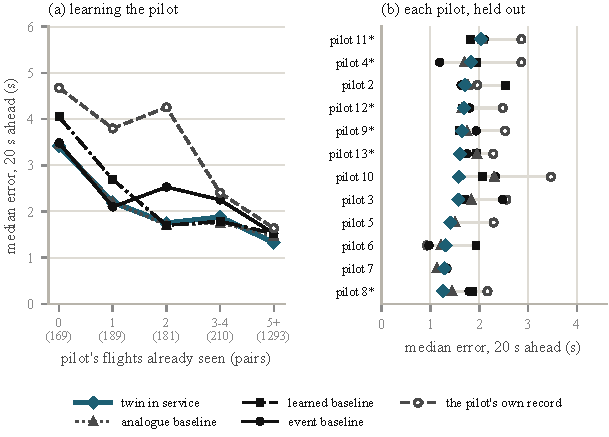
\includegraphics[width=\linewidth]{fig_prediction.pdf}
\caption{(a) Median error 20\,s ahead as a function of the number of the pilot's flights already seen, each pilot held out. (b) Each
pilot's median error 20\,s ahead; the twin is in colour.}
\label{fig:prediction}
\end{figure}

\subsection{What in a pilot's timing is personal}

Why does the pilot's own record help for some actions and not others? The intraclass correlation of a delay, the share of its variance
that lies between pilots rather than within one pilot's flights~\cite{shrout_fleiss_1979}, answers directly (Fig.~\ref{fig:signature}).
The pacing of routine actions is a personal signature. How long a pilot waits between the 50\,\% thrust stabilisation and take-off
thrust (0.71) and between brake release and take-off thrust (0.80) is stable from one flight to the next and differs between pilots, and
so, though less certainly, is the delay between gear up and the first flap retraction (0.75, with a wide interval). The response to a
failure is not: the delay between the failure and reverse thrust (0.00) and between reverse thrust and braking (0.02) is the same for
everyone, within each pilot's own variation. Gear up after liftoff is not personal either (0.02): its delay varies as much from one
flight to the next as from one pilot to another, in part because it shortens with practice (Section~\ref{sec:results}). A delay that
changes with experience cannot be a fixed signature.

\begin{figure}[t]
\centering
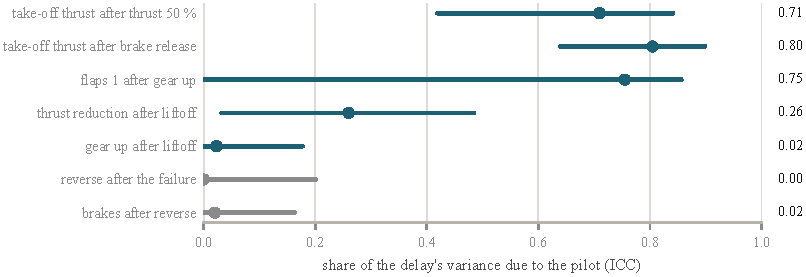
\includegraphics[width=\linewidth]{fig_signature.pdf}
\caption{Share of each delay's variance due to the pilot (intraclass correlation), twelve pilots, with 95\,\% intervals from a bootstrap
over pilots. Routine actions in colour, responses to a failure in grey.}
\label{fig:signature}
\end{figure}

\subsection{Flagging a missing action}

A twin that predicts an action can flag it when it is overdue: an alert is raised once the time read exceeds the latest prediction made
for the future by more than a margin learned on calibration pilots. On flights where the pilots made every action, the alerts are rare,
0.09 per flight. To test detection, we removed one key action at a time from what the mirror could see. Over the twelve pilots, 59\,\%
of these simulated omissions were flagged within 10\,s of the moment the action should have come, and 63\,\% when each pilot's delays were
personalised, against the 80\,\% we had set. The split is clean. With personalised delays, omissions of take-off thrust, thrust reduction
and reverse thrust were flagged in at least 96\,\% of cases, whereas gear up was flagged in 9 of 104 cases and the brakes of a rejected
take-off in 8 of 54.

%% ====================================================================================================
\section{Discussion}
\label{sec:discussion}

\paragraph{What the cognitive model adds.} A reader might expect a cognitive model to be needed to predict a pilot's next action, or
might suspect that it adds nothing a careful statistic could not. Our results support neither view. Much of what makes the twin better
than a pilot's own record is knowledge of the current flight, and a baseline that has that knowledge comes close at a short horizon. The
model's contribution is specific, and it holds for the model alone, without its blend with the reference: it predicts further ahead,
beyond the next event, and it transfers to a pilot it has never seen, because the structure of the procedure, which it holds, is shared
by all pilots while their timing is not. It also keeps every prediction
inspectable: the twin can say which task it expects, which constraint it is waiting for, and from which earlier action it counts. A
statistic that matches its error at ten seconds cannot say why.

\paragraph{Signature and response.} That routine pacing is personal and failure response is not has two consequences. For training, it
separates two kinds of measure: a tempo that is stable within a pilot, such as the pacing of the take-off roll, which characterises the
pilot, and delays that shorten with practice, such as gear up after liftoff, which track progress. The delay from liftoff to gear up of
the held-out pilots shrank from about 15 to 3\,s over their first ten flights (Section~\ref{sec:results}); a twin that errs by 1.5\,s
twenty seconds ahead can follow a change of that size. For
monitoring, an alert based on expectation can only be reliable for actions whose time is either personal and learned, or tightly cued by
an event. The critical actions of our corpus, gear up and the brakes of a rejected take-off, are neither, which is why the alerts missed
them. We also tried anchoring each alert on the event that triggers the action rather than on the clock; the anchor learned from one
group of pilots did not transfer to another, and the attempt failed its criterion. Only the brakes, anchored on reverse thrust, were
flagged reliably, and we have frozen that rule for the confirmatory study rather than adopt it after seeing the result.

\paragraph{What failed.} Several criteria failed, and four of the failures carry a lesson. The learning model's skill stopped improving after its
first flight in the frozen test, while it had not in development; a match that does not survive freezing is exactly what an evaluation of
digital human models should catch. The look-ahead predicted fewer of the pilots' actions than the reference did, which the weighted
average corrects only by construction. The cognitive state we estimate from physiology and behaviour changed the model's predictions
but did not improve them: with the random seed of ACT-R held equal, the difference was $+0.012$\,s (95\,\% interval $-0.012$ to
$+0.036$). And the alerts fell short, for the reason given above.

\paragraph{Threats to validity.} Twelve pilots are few. A majority of seven is weak evidence, and only a result such as 11 of 12 is
strong on its own; we report both the count of pilots and an interval over pilots for that reason. The held-out pilots had been seen by
the time several corrections were made, and the cross-validated comparisons of Section~\ref{sec:own} were designed after an earlier
attempt had failed; they are exploratory, however honest the estimation within them. The twin's own parameters were set on the
calibration pilots, so for those six pilots the twin is not fully held out; restricted to the six validation pilots, the result is 5 of
6 against the event baseline. The mirror was checked against an offline reading of the same flights, which applies the same procedural
knowledge through a separate program, and, for take-off thrust, rotation and gear up, against an extraction made independently of
our work; no flight was annotated by hand. Omissions were simulated by hiding an action that the pilot did make, so the rest of the
flight is that of a pilot who did not forget. The pilots flew an A320 on a fixed-base simulator; only the learning test involves our agent's own flying,
which is on an A330, and that test compares quantities that do not depend on the aircraft type. Finally, the data cannot be released,
which limits replication to the protocol and the reported statistics.

\paragraph{Next.} The decisive test is prospective. A study with new pilots, each flying twelve take-offs with failures, is planned;
before any of its data exist, we have frozen the version of the twin it will test and three criteria: that the twin beats each pilot's
own record, that it beats the event baseline at 20\,s, and that the pacing of the routine, but not the response to a failure, is a
personal signature.

%% ====================================================================================================
\section{Conclusion}

The same declarative knowledge that lets an ACT-R pilot fly a procedure lets it read a pilot's flight against that procedure and
anticipate the pilot's next actions. On twelve pilots, each predicted without being learned from, the twin anticipates a pilot's actions
better than the pilot's own record, and better than the strongest statistical baseline we could build when it looks twenty seconds
ahead. The pacing of routine actions is personal, the response to a failure is not. These results come with their failures, which we
have kept in view: a model whose learning plateaued, alerts that miss the actions that matter most, and a cognitive state that does not
help prediction. A confirmatory study with new pilots will tell which of these findings hold.

\subsubsection*{Acknowledgments.} This work is part of a research partnership with industrial partners who provided the simulator data
and the procedure ontology. An AI coding assistant was used to write analysis scripts; every number in this paper is recomputed from the
data by scripts kept with the paper.

\subsubsection*{Disclosure of Interests.} The authors have no competing interests to declare that are relevant to the content of this
article.

\bibliographystyle{splncs04}
\bibliography{references}

\end{document}
